\documentclass[12pt]{article}
\usepackage{amsmath}
\usepackage{graphicx}
\usepackage{hyperref}
\usepackage[latin1]{inputenc}

\title{Getting started}
\author{Veloci Raptor}
\date{03/14/15}

\begin{document}
\maketitle

Welcome to LaTeX Base, a web-based \LaTeX{} editor with live document preview!
Here are some things to try --

\begin{itemize}
  \item edit the document name above by typing in the input field
  \item make changes to the body on the left and watch the preview update
  \item include an image by url like this one
        \hspace*{3em}
        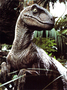
\includegraphics{raptor.jpg}
  \item check the compiler output by clicking the log button
  \item format a mathematical expression like
        $\frac{1}{2\pi}\int_{-\infty}^{\infty}e^{-\frac{x^2}{2}}dx$
  \item download the document as a pdf by selecting Export $>$ Local
        Filesystem (or by clicking the desktop download button)
  \item export your work to Dropbox or Google Drive
  \item import an existing document from your local computer
  \item try using the vim or emacs keyboard shortcuts
\end{itemize}

Editing short documents online is free. View premium plans and pricing at
\url{https://latexbase.com/static/pricing} to enjoy unlimited document editing
(online or offline) and a variety of other useful features. Thanks for trying
out our service and don't hesitate to get in touch at
\href{mailto:support@latexbase.com}{support@latexbase.com}!

\end{document}
